% !TeX root = ../thesis.tex

\section{Design Goal}
\subsection{Hardware Build}
The idea is to use \glspl{IC} of the well known 74 series for the logic functionality.
Initially, it was planned to build the \gls{CPU} similar to the 8-bit CPU project by Ben Eater \cite{eater_cpu} out of breadboards.
However, breadboards make for great prototyping but are known for their not-ideal connectivity and wires can come loose quite easily.
Especially when using about 15 boards errors due to bad connections are prone to happen.
On the other side, the proper approach would be to design a \gls{PCB} for the \gls{CPU}.
I decided against it for two main reasons:\\
I had little to no experience designing \glspl{PCB}, from layouting to placing and routing.
Additionally, I never worked with the 74 series \glspl{IC} and wanted to work with them in an easier to change environment similar to breadboards.
Secondly, designing such a large \gls{PCB} would have been very costly compared to what my financial plans for this project were.

\begin{figure}[t]
  \centering
  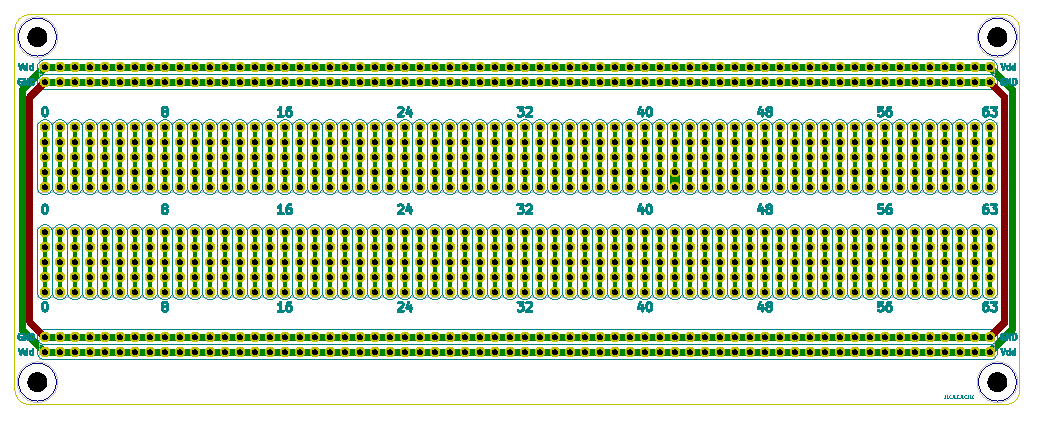
\includegraphics[width=\textwidth]{breadboardPcb.pdf}
  \caption{\gls{PCB} used for the hardware built of the first version of the \gls{CPU}.}
  \label{fig:breadboardPcb}
\end{figure}
Therefore, I decided to find a solution in the middle: A more permanent solution than breadboards but not already fully wired on a big \gls{PCB}.
I designed a small \gls{PCB} that is very similar to a breadboard with some minor tweaks to make it better suited for my goal.
It is shown in \cref{fig:breadboardPcb}.
I could order 25 of these boards from JLCPCB\footnote{\url{https://jlcpcb.com}} for only 34 USD shipped to Germany making it by far the cheapest option.

\begin{table}
  \centering
  \renewcommand{\arraystretch}{1.25}
  \caption{All logic \glspl{IC} used in the first \gls{CPU} version.}
  \label{tab:cpuIcs}
  \begin{tabularx}{\textwidth}{ |l|c||X| }
    \hline
    Quantity & \gls{IC}       & Function                                 \\\hline\hline
    23       & 74LS157        & quad 2 to 1 multiplexer                  \\\hline
    11       & 74LS08         & quad AND gate                            \\\hline
    9        & 74LS86         & quad XOR gate                            \\\hline
    6        & 74LS32         & quad OR gate                             \\\hline
    6        & 74LS374        & octal register (tri-state output)        \\\hline
    5        & 74LS245        & octal bus transceiver (tri-state output) \\\hline
    4        & 74LS273        & octal register with asynchronous clear   \\\hline
    4        & NA555P         & 555 timer                                \\\hline
    3        & 74LS00         & quad NAND gate                           \\\hline
    3        & 28C64          & 32k x 8 bit EEPROM (tri-state output)    \\\hline
    1        & AS6C1008-55PCN & 128k x 8 bit SRAM (tri-state output)     \\\hline
  \end{tabularx}
\end{table}
\begin{figure}[t]
  \centering
  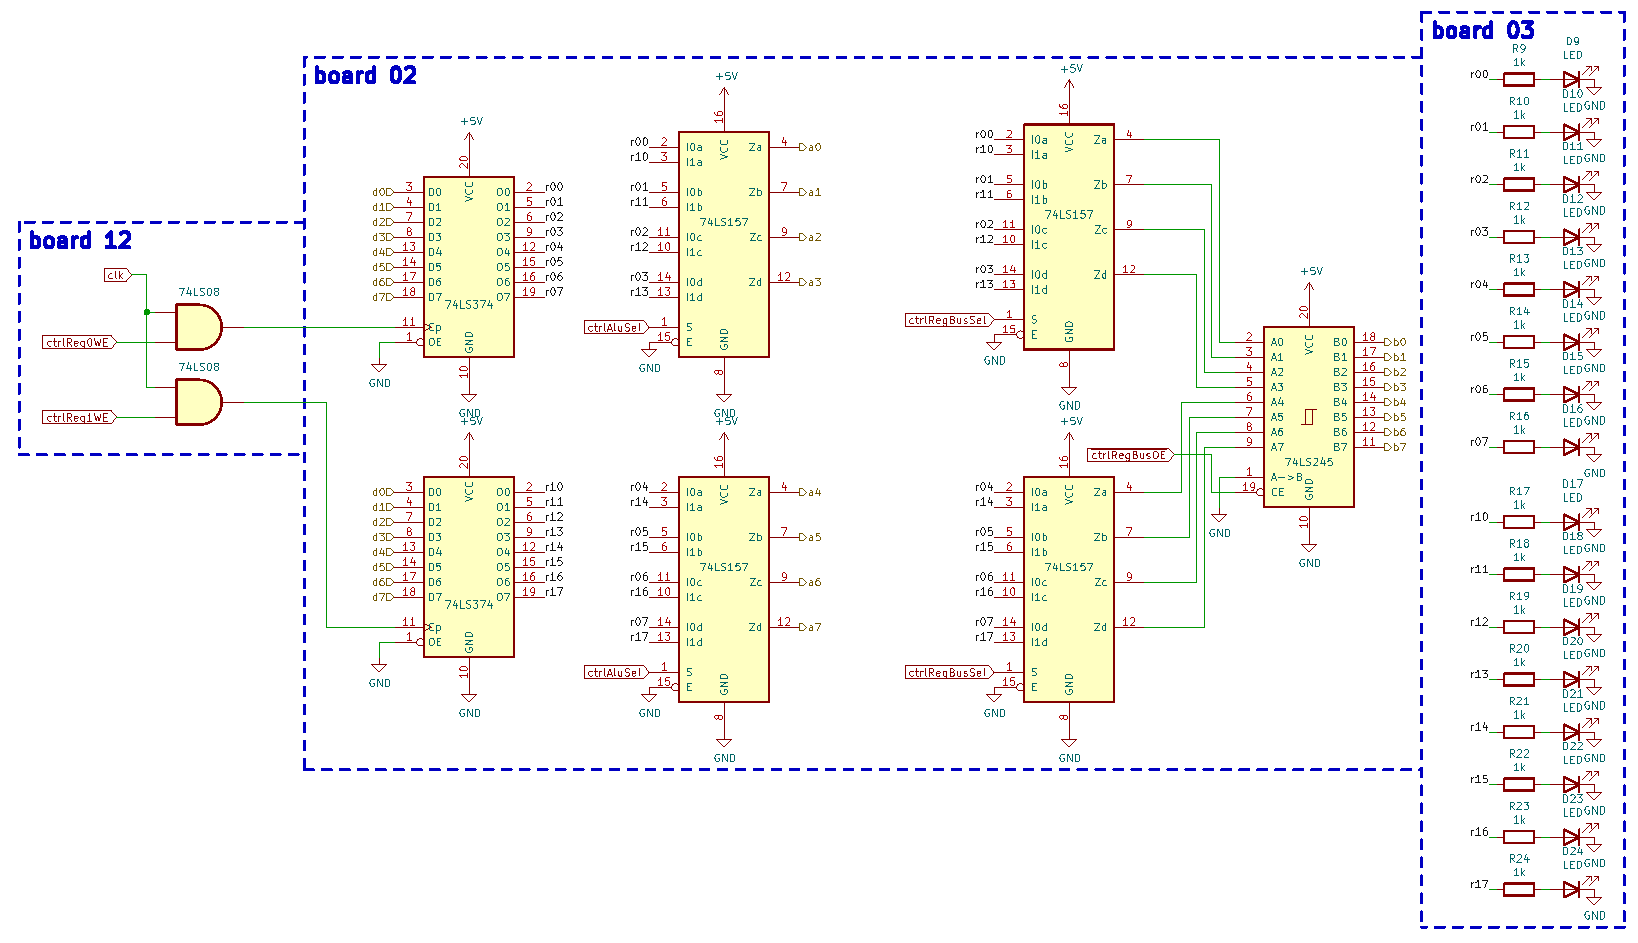
\includegraphics[width=\textwidth]{regset.pdf}
  \caption{Register File with two general purpose register, \gls{ALU} A input, bus driver and LEDs.}
  \label{fig:regset}
\end{figure}
The logic \glspl{IC} that have been used in the \gls{CPU} are listed in \cref{tab:cpuIcs}.
To make it easier to debug and also to visualize what the \gls{CPU} is calculating, most registers have \glspl{LED} attached to their outputs via resistors.
The layout of the register file is shown in \cref{fig:regset} as an example.
It can be seen that one breadboard-like \gls{PCB} holds 7 logic \glspl{IC} and the \glspl{LED} were placed on another board.
The clock pulse of the registers (\texttt{r0/1\_cp}) comes from another board where the clock has been ANDed with multiple \texttt{clockEnable} control signals (not all shown).
Problems of this kind of design and also how they were resolved for the \gls{EDiC} is presented in \cref{sec:improvements}.

\subsubsection{Clock Module}
\begin{figure}[t]
  \centering
  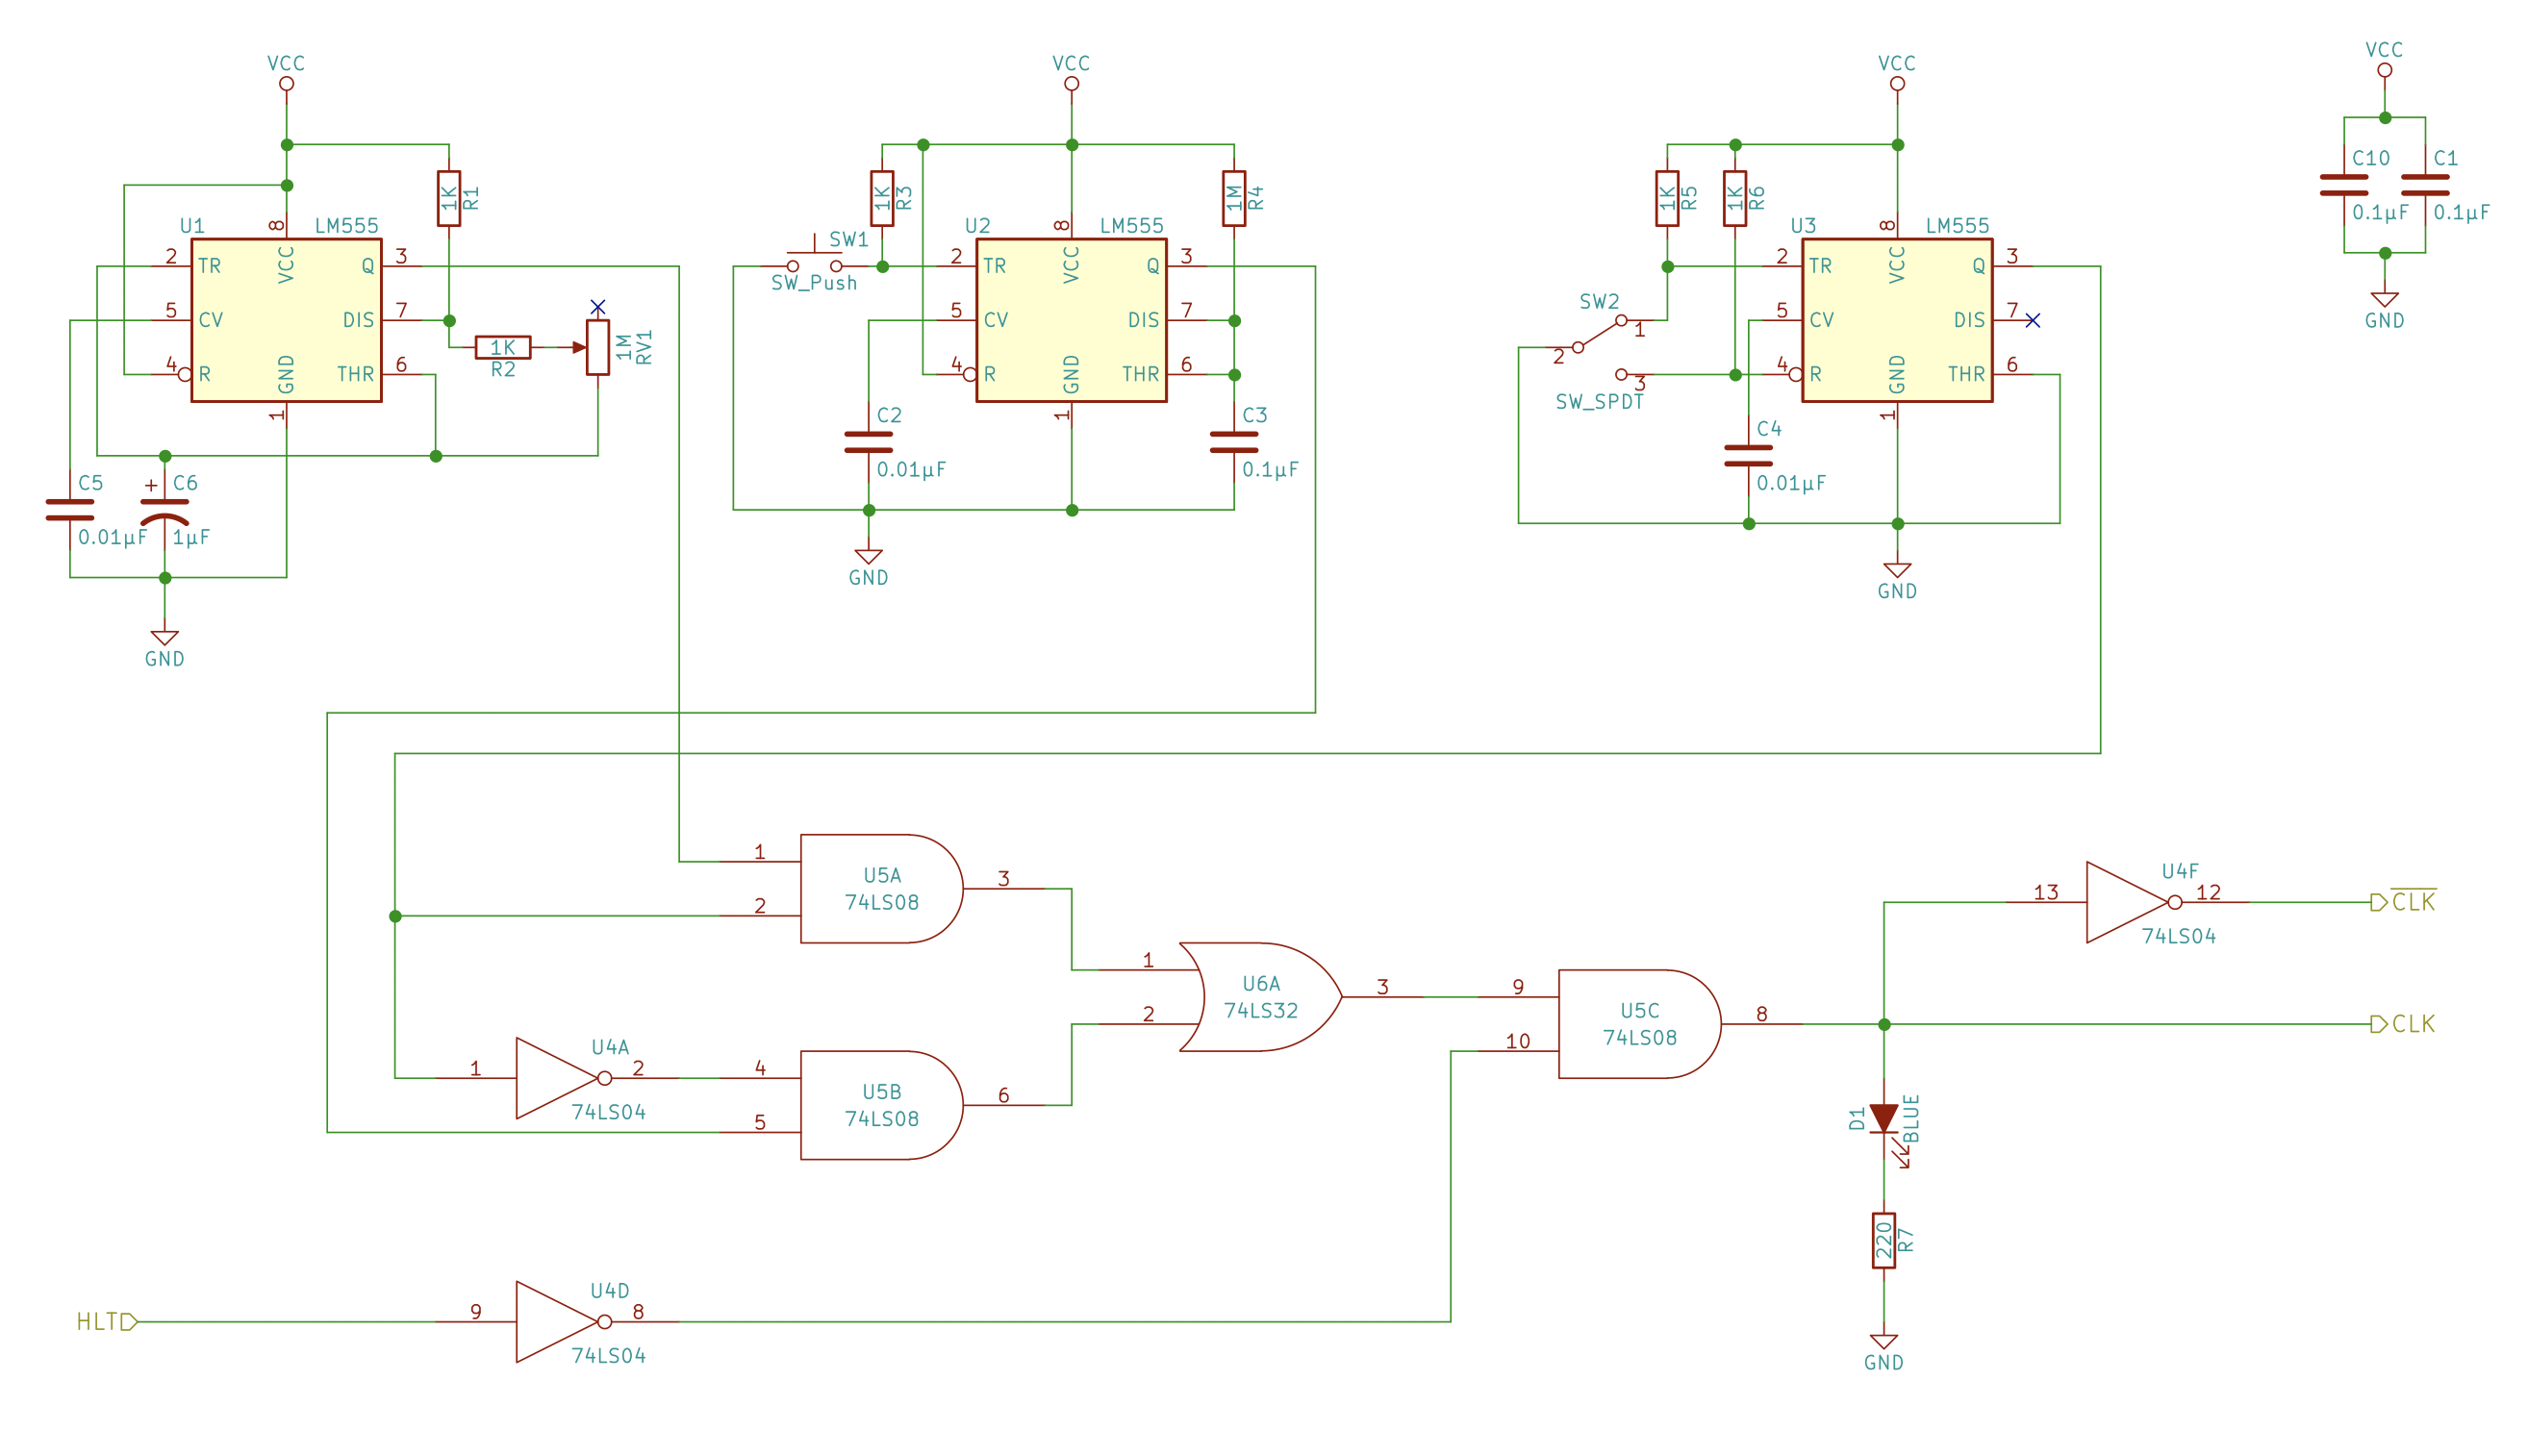
\includegraphics[width=\textwidth]{eater_clock.png}
  \caption{The schematic of the clock module by Ben Eater \cite{eater_clock} which inspired the clock module of the first version of the \gls{CPU}.}
  \label{fig:eater_clock}
\end{figure}
One clock module which cannot be simulated as well as the others is the clock module.
Its circuit is heavily inspired by the clock module of the above mentioned series by Ben Eater \cite{eater_clock} which exploits three possible use cases of the well known 555 timer.
The 555 timer \gls{IC} is a massively used \gls{IC} which features voltage dividers, two comparator, one SR flip-flop, an output driver and a discharge transistor \cite{LoweDoug555}.
As shown in \cref{fig:eater_clock} the three use cases for the 555 timer are in the astable (left), monostable (middle) and bistable (right) configuration.

The astable configuration works by charging C6 over R1, R2 and RV1 until a upper threshold voltage is reached which resets the internal flip-flop.
This allows the capacitor to discharge to the 555 internal ground until a lower threshold is reached and the flip-flop is set again to recharge the capacitor.
Depending on the capacitor and resistor dimensions this creates a never ending cycle of sets and resets of the flip-flop and in combination with the output buffer a clock.
By using a potentiometer as RV1 it is possible to control the clock frequency\footnote{The duty cycle of the clock is also affected but for the low frequencies I used this circuit (<1kHz) this has no effect on the logic circuit.}.

The monostable configuration is used to debounce a button press to be used for stepping the clock one cycle at a time.
It creates an active high pulse when the button is pressed once. All consecutive button presses (or bounces) only prolong the pulse but do not trigger another pulse.
If the button press would not be debounced it is possible that one press of the button results in multiple edges on the clock line which in turn can result in undefined and unknown behavior.
This was a cause for a small bug in the commissioning of the \gls{EDiC} as presented in \cref{sec:commissioning}.

The bistable configuration is used to switch between the two clock sources (astable and monostable).
It also uses the internal flip-flop to debounce the switch.

The lower logic gates are used to multiplex the two clock sources and additionally halt the clock when such an instruction is executed.
